\chapter{Identificação e Controle}
\label{cap:id-e-controle}

Para a execução de um algoritmo que permita o robô \textit{micromouse} se locomover dentro do esperado faz-se necessário compreender que existem diferenças mecânicas nos motores que influenciam diretamente o comportamento global do robô e apenas contornando tais diferenças será possível obter o desempenho desejado. E, dessa forma, entra em cena a Teoria de Controle para fazer com que, apesar das suas diferenças, os motores possam ao fim ter comportamentos semelhantes (ou iguais, o caso ideal).


    \section{Identificação de Sistemas Dinâmicos} \label{sec:id-teoria}
		
		Inicialmente faz-se necessário conceituar o que é um sistema,  o qual é o objeto de estudo dentro do controle. Assim, um sistema é entendido por \citeonline{coelho-identificacao} como um conjunto de objetos que realizam um determinado fim, podendo ser físico, biológico, químico ou outro. 
		
		Entre os sistemas dinâmicos os \textit{processos} mais comuns são os de velocidade, de temperatura e de nível. Cada um desses tipos tem características próprias que os diferenciam dos demais, ao mesmo tempo que possuem, também, elementos em comum e que permitem a sua generalização teórica. Um exemplo de sistema pode ser visto na Figura \ref{fig:sistema-controle-generico}.

		\begin{figure}[htbp]
				\centering
				\Caption{\label{fig:sistema-controle-generico} Exemplo de um sistema genérico}	
				\UFCfig{}{
					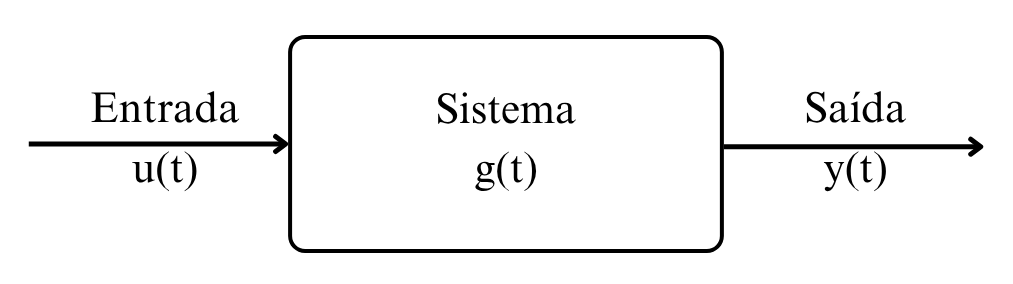
\includegraphics[width=8cm]{figuras/fundamentação-teorica/exemplo-sistema.png}
				}{
					\Fonte{O autor}
				}	
		\end{figure}

		Outra característica a ser considerada dentro dos sistemas estudados tem a ver com a sua linearidade ou não, ou seja, a possibilidade de se aplicar o princípio da superposição no processo analisado, visto que a resposta a diversas entradas simultâneas pode ser entendida como a soma das respostas a cada entrada individualmente \cite{ogata-2010}.

		Processos de velocidade, tais quais os dos motores presentes no \textit{micromouse}, apresentam não linearidades inerentes ao sistema. Porém, como mostrado em \citeonline{dissetacao-pereira-2000}, para o caso dos micro-robôs móveis com equações cinemáticas como as descritas em \ref{eq:vel-linear-global} a \ref{eq:vel-linear-esquerda}, as não linearidades são consideradas fracas de maneira que os parâmetros do modelo ainda são lineares.

		\subsection{Modelagem em domínio contínuo} \label{ssec:modelagem-domniio-continuo}

			Uma forma comum para descrever sistemas consiste na sua modelagem matemática. Assim, supondo que $g(t)$ seja uma função matemática de tempo contínuo capaz de modelar a dinâmica do sistema, e que os sinais de entrada e de saída do sistema, respectivamente $u(t)$ e $y(t)$, possuam suas Transformadas de Laplace $U(s)$ e $Y(s)$, pode se representar o bloco da Figura \ref{fig:sistema-controle-generico} pela equação \ref{eq:funcao-transferencia-generica-s} a qual é definida como \gls{FT} do sistema em tempo contínuo.

			\begin{equation}
				\label{eq:funcao-transferencia-generica-s}
				G(s) = \frac{Y(s)}{U(s)} = \frac{\mathcal{L}\{y(t)\}}{\mathcal{L}\{u(t)\}}
			\end{equation}
			
			A Equação \ref{eq:funcao-transferencia-generica-s} pode ser expandida para a forma da Equação \ref{eq:expansao-ft-s}, onde $b_i$ e $a_i$ são os coeficientes polinomiais de $Y(s)$ e $U(s)$ respectivamente. O sistema pode então ser dito de \textit{ordem n} caso a maior potência do seu denominador seja $n$ \cite{ogata-2010}.

			\begin{equation}
				\label{eq:expansao-ft-s}
				G(s) = \frac{Y(s)}{U(s)} =\frac{b_0 s^m + b_1 s^{m-1} + \cdots + b_{m-1} s + b_m}{a_0 s^n + a_1 s^{n-1} + \cdots + a_{n-1} s + a_n}
			\end{equation}

			Os sistemas na natureza, entretanto, podem ser modelados por \gls{FT} de ordem $2$. Dessa forma, que a Equação \ref{eq:expansao-ft-s} pode ser agora reduzida a Equação \ref{eq:ft-ordem-2-s}.

			\begin{equation}
				\label{eq:ft-ordem-2-s}
				G(s) = \frac{Y(s)}{U(s)} =\frac{b_1 s + b_2}{s^2 + a_1 s + a_2}
			\end{equation}

		\subsection{Modelagem em domínio discreto} \label{ssec:modelagem-domniio-discreto}

			Sistemas computacionais, por sua vez, não são capazes de compreender fenômenos contínuos haja vista que a sua natureza binária e digitalizada não os permite de suportar os infinitos valores em um intervalo finito e real e, portanto, é necessário converter os modelos descritos anteriormente em modelos discretos através da Transformada $Z$. A Transformada $Z$ é aplicada não ao sinal original, mas ao sinal amostrado a partir de um intervalo de tempo $T_s$. 
			
			Assim, dado um sinal genérico $r(t)$ e amostrado no intervalo de tempo $T_s$, conforme a Figura \ref{fig:amostragem-tempo-discreto}, pode-se definir a transformada $Z$ do sinal conforme \citeonline{ibrahim-2006}, pela Equação \ref{eq:definicao-transformada-z}.

			\begin{figure}[htbp]
					\centering
					\Caption{\label{fig:amostragem-tempo-discreto} Amostragem de um sinal contínuo}	
					\UFCfig{}{
						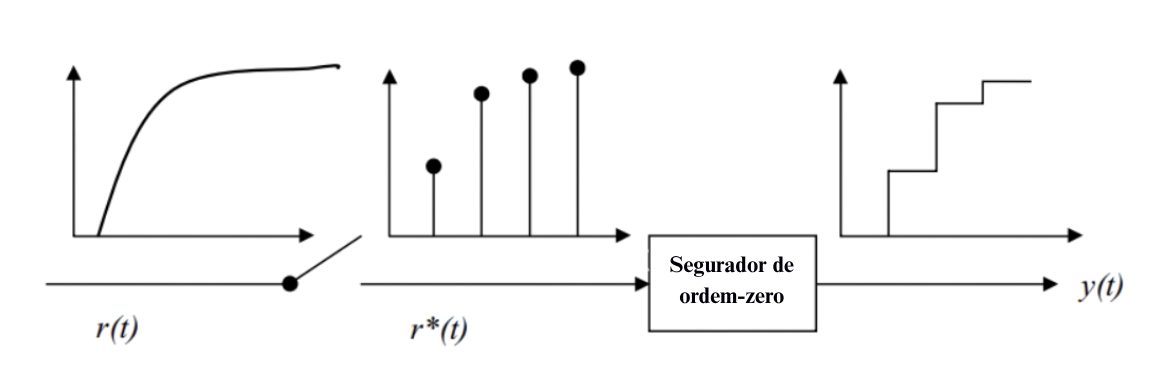
\includegraphics[width=9cm]{figuras/fundamentação-teorica/amostragem-ibrahim.png}
					}{
						\Fonte{\citeonline{ibrahim-2006}}
					}	
			\end{figure}

			\begin{equation}
				\label{eq:definicao-transformada-z}
				Z[r(t)] = R(z) = \sum_{n=0}^{\infty} r(n T_s) z^{-n}
			\end{equation}

			Aplicando a equação anterior na \gls{FT} dos processos de segunda ordem descritos pelo Equação \ref{eq:ft-ordem-2-s}, pode-se obter a \gls{FT} discreta conforme \ref{eq:ft-ordem-2-z}. 

			\begin{equation}
				\label{eq:ft-ordem-2-z}
				G(z) = \frac{Y(z)}{U(z)} = \frac{b_1 z^{-1} + b_2 z^{-2}}{z + a_1 z^{-1} + a_2 z^{-2}}
			\end{equation}

			Em sistemas reais as resposta não são instantâneas, de modo que pode existir um certo intervalo de tempo até que seus efeitos sejam visíveis, e, dessa forma, faz-se necessário considerar o termo do \textit{atraso de transporte}, fazendo com que a forma final usada para modelagem de sistemas dinâmicos seja a Equação \ref{eq:ft-ordem-2-z-com-atraso}.

			\begin{equation}
				\label{eq:ft-ordem-2-z-com-atraso}
				G(z) = \frac{Y(z)}{U(z)} = z^{-d} \frac{b_1 z^{-1} + b_2 z^{-2}}{z + a_1 z^{-1} + a_2 z^{-2}}
			\end{equation}
			
			\noindent
			onde os termos $z^{-1}$, $z^{-2}$ e $z^{-d}$ indicam atrasos de 1, 2 e $d$ \textit{períodos amostragem} respectivamente.

			Assim, a \textit{equação a diferenças} usada para os cálculos computacionais é derivada a partir da \gls{FT} discreta do processo e está explicitada na Equação \ref{eq:equacao-diferencas}.

			\begin{equation}
				\label{eq:equacao-diferencas}
				y[k] = -a_1 y[k-1] - a_2 y[k-2] + b_1 u[k-1-d] + b_2 u[k-2-d]
			\end{equation}

			As Equações \ref{eq:ft-ordem-2-z-com-atraso} e \ref{eq:equacao-diferencas} serão usadas para a construção do vetor de parâmetros para a estimação do modelo.

		\subsection{Estimador dos Mínimos Quadrados Não-Recursivo} \label{ssec:estimador-mqnr}

			O Estimador dos \gls{MQNR} é uma técnica clássica baseada no \textit{Princípio dos Mínimos Quadrados} de Gauss elaborado no século XVIII para prever as trajetórias de planetas a partir da realização de medições e observações \cite{coelho-identificacao}. 
			
			Este método utiliza um vetor de medidas, $\varphi(t)$, a partir de um conjunto de dados extraídos de experimentações para a construção de uma aproximação $\hat{\theta}$ do vetor de parâmetros $\theta(t)$ do qual os elementos são retirados e utilizados diretamente na Equação \ref{eq:equacao-diferencas}.

			O vetor das medidas coletadas, $\varphi(t)$, com dimensão $[(m + n + 1) \times 1]$, é definido pela Equação \ref{eq:vetor-phi-medidas}.

			\begin{equation}
				\label{eq:vetor-phi-medidas}
				\varphi^T(t) = [-y(t-1) \ -y(t-2) \ \ldots \ -y(t-m) \ u(t-d) \ \ldots \ u(t-d-n)]
			\end{equation}

			Já o vetor de parâmetros, $\hat{\theta}$, é:
			\begin{equation}
				\label{eq:vetor-theta-medidas}
				\theta^T(t) = [a_1 \ a_2 \ \ldots \ a_{m} \ b_0 \ b_1 \ \ldots \ b_{n}]
			\end{equation}

			E a representação matricial da saída do sistema é dada por:

			\begin{equation}
				\label{eq:vetor-y-medidas}
				Y = \Phi \theta + E
			\end{equation}

			\noindent
			onde $E$ é o vetor de pertubações e $\Phi$ a matriz para $N$ medidas, dada por \ref{eq:matriz-Phi-medidas}.

			\begin{equation}
				\label{eq:matriz-Phi-medidas}
				\Phi =  \begin{bmatrix}
							\varphi^T(0) \\
							\varphi^T(1) \\
							\vdots \\
							\varphi^T(N-1)
						\end{bmatrix}
			\end{equation}
			
			O critério para obtenção do vetor de parâmetros $\hat{\theta}$ é dado pela resolução da Equação \ref{eq:criterio-minimizacao-mqnr} a qual corresponde à minização do erro de previsão quadrático.

			\begin{equation}
				\label{eq:criterio-minimizacao-mqnr}
				J = \min_{\theta} \left\| Y - \phi \hat{\theta} \right\|_W^2
			\end{equation}

			Assim, resolvendo a equação anterior é possível obter a definição de $\hat{\theta}$.

			\begin{equation}
				\label{eq:estimador-mqnr}
				\hat{\theta} = [\Phi^T \Phi]^{-1} \Phi^T \mathbf{Y}
			\end{equation}

			Para que a estimação dos parâmetros seja a mais precisa possível, \citeonline{dissetacao-pereira-2000} estabelece que a aquisição de dados deve considerar 3 pontos, os quais são:

			\begin{enumerate}
				\item A coleta de dados deve ser em malha aberta para evitar a correlação entre as entradas.
				\item O sistema deve ser excitado de forma a extrair o máximo possível da informação da panta.
				\item A excitação deve ser feita com pequenas variações em torno de um ponto de operação a fim de reduzir o efeito de fenômenos não modelados como não linearidades.
			\end{enumerate}

			Em consonância com o estabelecido acima, \citeonline{aguirre-identificacao-2007} estabelece que o sinal de entrada deve ser um sinal branco. Isto implicará que tal sinal tem energia em uma faixa de frequências ampla e que engloba a faixa de frequências dominantes do sistema que se deseja identificar, ou seja, o sinal branco será capaz de excitar adequadamente a dinâmica da planta, o que pode ser obtido quando a excitação ocorre em torno de um ponto de operação.

			Conjuntamente deve ser observado também que o produto matricial $[\Phi^T \Phi]$, presente na Equação \ref{eq:estimador-mqnr}, deve ser invertível. Assim, supondo o sinal de entrada, $u(t)$, constante e igual a $u_0$, tem-se, para $N$ medidas, que o produto resultará em uma matriz singular no formado de:

			\begin{center}
				$
				[\Phi^T \Phi] = N u_0 
				\begin{bmatrix}
					1 & 1 \\
					1 & 1 \\	
				\end{bmatrix}
				$
			\end{center}

			E, portanto, o sinal de entrada deve possuir variação para garantir que a Equação \ref{eq:determinante-nao-nulo} seja obedecida.

			\begin{equation}
				\label{eq:determinante-nao-nulo}
				\text{det} \left\{ \Phi^T \Phi \right\} \neq 0
			\end{equation}

			Desse modo, a escolha do sinal de entrada adequado é crucial para a correta identificação de sistemas de controle. Um dos sinais mais empregados nesse contexto é o \gls{PRBS}, conforme apresentado por \citeonline{aguirre-identificacao-2007}, \citeonline{coelho-identificacao} e \citeonline{norgaard-2000-neural}, devido à sua capacidade de atender aos requisitos descritos anteriormente.

			% Desse modo a escolha do sinal de entrada adequado é crucial para a correta identificação dos sistemas de controle. Um dos sinais mais comumente empregados nesse contexto são os \gls{PRBS} os quais além de aparecerem em \cite{aguirre-identificacao-2007, coelho-identificacao, dissetacao-pereira-2000} também são apresentados em \citeonline{norgaard-2000-neural} devido à sua capacidade de atender a todos os requisitos descritos anteriormente.

			Sinais \gls{PRBS} são sequências pseudo-aleatórias que podem assumir apenas dois valores em torno de um ponto de operação. Tais sinais são determinísticos, isto é, podem ser gerados novamente diversas vezes, são periódicos com metade mais um dos intervalos em um nível e, metade menos um, em outro nível \cite{aguirre-identificacao-2007}.
			
			Assim, diante do exposto até aqui, o presente trabalho faz uso do referido sinal como sinal de entrada para modelagem dos sistemas dinâmicos presentes no \textit{micromouse}, a saber:

			\begin{itemize}
				\item O robô, quanto ao seu comportamento relativo à sua velocidade linear global, descrito pela Equação \ref{eq:vel-linear-global}.
				\item O robô, quanto ao seu comportamento relativo à sua velocidade angular global, descrito pela Equação \ref{eq:vel-angular-global}.
				\item Os motores de corrente contínua, responsáveis pelas velocidades direita e esquerda do robô, os quais são descritos pelas Equações \ref{eq:vel-linear-direita} e \ref{eq:vel-linear-esquerda}, respectivamente.
			\end{itemize}
				
    \section{Controle de Sistemas Dinâmicos} \label{sec:controle-teoria}

        % \textbf{abordar aqui: relé, astrom, PID e Equações do PID em Z}
		
		De posse do modelo de cada um dos sistemas, elaborados conforme as seções anteriores, é possível proceder para o projeto e desenvolvimento dos controladores. Este trabalho faz uso de controladores do tipo \gls{PID} projetados utilizando o método de {\AA}str{\"o}m com autossintonia pelo Método do Relé. Todo o processo é realizado computacionalmente, ou seja, é feito também o uso da \textit{Transformada Z} descrita em \ref{eq:definicao-transformada-z}.

		\subsection{Controlador Proporcional-Integral-Derivativo} \label{ssec:teoria-pid}

			Até agora, os sistemas considerados encontravam-se em \gls{MA}, como o exemplo mostrado na Figura \ref{fig:sistema-controle-generico}, isto é, era aplicado um sinal de entrada $u(t)$ e era observado o comportamento da saída $y(t)$. Entretanto, controlar um sistema significa forçar o seu comportamento final para um comportamento desejado de forma que, na maioria das vezes, isso deve ser realizado com a utilização de uma realimentação, o que qualifica o sistema agora como em \gls{MF}, pois está presente, também, um sinal de referência $r(t)$ e um sinal de erro $e(t)$ definido como:

			\begin{equation}
				\label{eq:definicao-erro}
				e(t) = r(t) - y(t)
			\end{equation}

			A Figura \ref{fig:sistema-malha-fechada-simples} exemplifica um sistema em \gls{MF} e a Figura \ref{fig:sistema-malha-fechada-controlador} exemplifica um sistema em \gls{MF} controlado. A partir da Figura \ref{fig:sistema-malha-fechada-controlador} pode-se observar que o controlador irá atuar em cima do erro $e(t)$ de forma que o objetivo é zerar o valor desse sinal.

			\begin{figure}[htpb]
				\centering
				\Caption{\label{fig:sistema-malha-fechada-simples} Sistema em Malha Fechada}
				\UFCfig{}{
					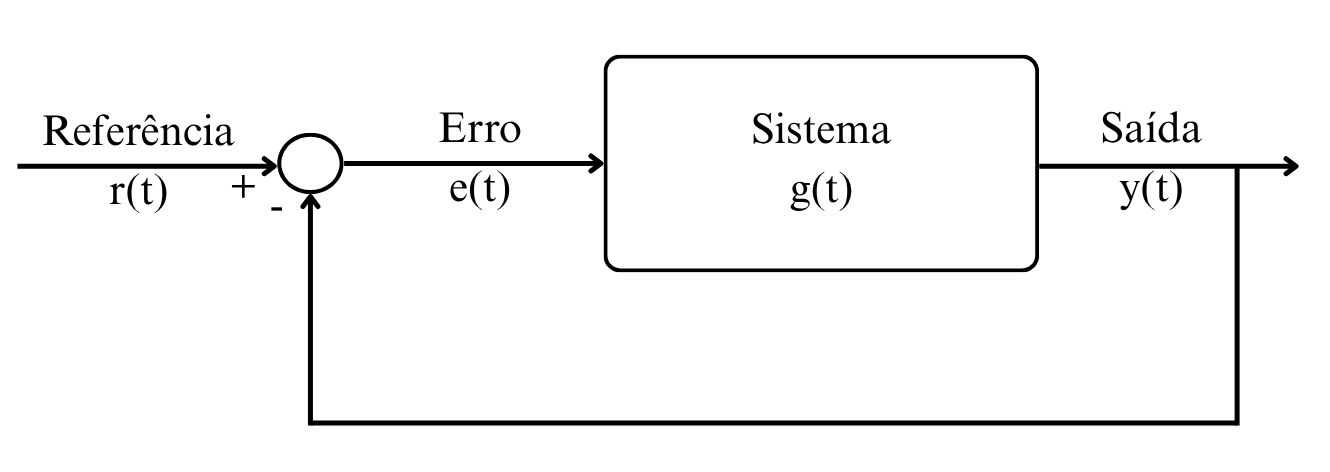
\includegraphics[width=12cm]{figuras/fundamentação-teorica/sistema-mf-simples.png}
				}{
					\Fonte{O autor}
				}	
			\end{figure}

			\begin{figure}[htpb]
				\centering
				\Caption{\label{fig:sistema-malha-fechada-controlador} Sistema em Malha Fechada com Controlador}
				\UFCfig{}{
					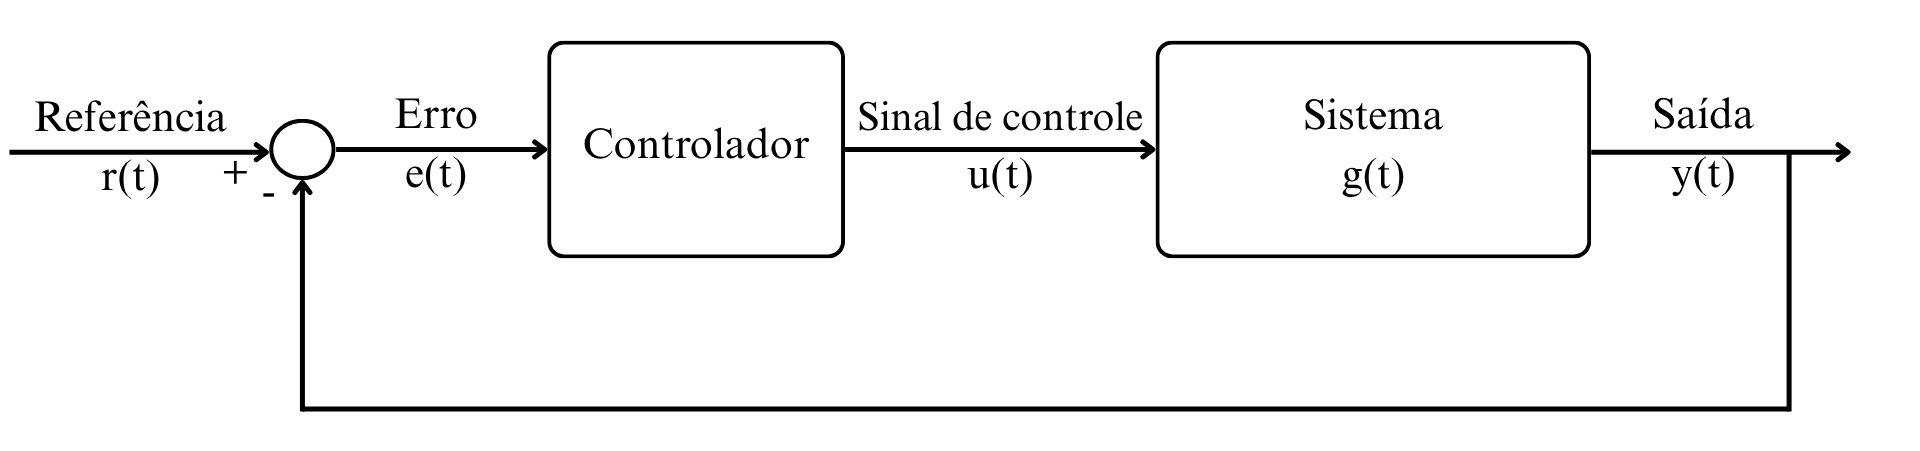
\includegraphics[width=12cm]{figuras/fundamentação-teorica/sistema-mf-controlado.png}
				}{
					\Fonte{O autor}
				}	
			\end{figure}
			
			Assim, o controlador \gls{PID}, definido pela Equação \ref{eq:definicao-pid-tempo}, é composto de três tipos básicos de ação de controle: a ação proporcional, a ação integrativa e a ação derivativa. A ação proporcional consiste em um ganho (chamado de ganho proporcional) simples aplicado ao erro, visando reduzir valor do \textit{erro de regime permanente}. A ação integrativa consiste em um ganho (ganho integrativo) aplicado à soma do erro em um intervalo de tempo $t$, seu objetivo é zerar o \textit{erro de regime permanente}. Por fim, a ação derivativa consiste em um ganho (ganho derivativo) aplicado à taxa de variação do erro em um intervalo de tempo $t$, cujo objetivo é corrigir problemas no transitório da resposta do sistema. 
			
			\begin{equation}
				\label{eq:definicao-pid-tempo}
				u(t) = K_p e(t) + K_i \int_0^t e(t) \, dt + K_d \frac{de(t)}{dt}
			\end{equation}

			\noindent
			onde $K_p$, $K_i = \frac{K_p}{T_i}$ e $K_d = K_p T_d$ são os ganhos proporcional, integrativo e derivativo respectivamente. $T_i$ representa o tempo de integrativo e $T_d$ representa o tempo de derivativo. E, aplicando a \textit{Transformada de Laplace} na equação anterior, é possível obter a \gls{FT} em $s$ de um controlador \gls{PID}.

			\begin{equation}
				\label{eq:definicao-pid-laplace}
				G_c(s) = \frac{U(s)}{E(s)} = K_p \left( 1 + \frac{1}{T_i s} + T_d s \right)
			\end{equation}
			
			Assim, ao aplicar-se a \textit{Transformada Z}, para uma amostragem com um período de amostragem $T_s$, na Equação \ref{eq:definicao-pid-laplace}, obtêm-se a \gls{FT} em $z$ de um controlador \gls{PID}, a qual é definida por:

			\begin{equation}
				\label{eq:definicao-pid-z}
				G_c(z) = \frac{U(z)}{E(z)} = \frac{g_0 z^2 + g_1 z + g_2}{z(z-1)}
			\end{equation}

			\noindent
			onde,

			\begin{center}
				$g_0 = K_p + \frac{K_i T_s}{2} + \frac{K_d}{T_s}$ \\
				$g_1 = \frac{K_i T_s}{2} - K_p - \frac{2 K_d}{T_s}$ \\
				$g_2 = \frac{K_d}{T_s}$
			\end{center}

			E, por fim, a equação a diferenças do controlador \gls{PID} obtida a partir de \ref{eq:definicao-pid-z} é:

			\begin{equation}
				\label{eq:equaca-diferenca-pid}
				u[k] = g_0 e[k] + g_1 e[k-1] + g_2 e[k-2] + u[k-1]
			\end{equation}

			De posse das equações acima, o passo seguinte é sintonizar os parâmetros $K_p$, $T_i$ e $T_d$.

		\subsection{Sintonia pelo Método do Relé} \label{sec:autossintonia-rele}

			A escolha dos parâmetros do controlador \gls{PID} não é um processo trivial ou intuitivo e, a depender da abordagem escolhida, demanda testes experimentais (podendo ser simulados com o uso do modelo) ou um desenvolvimento matemático analítico mais completo. Técnicas clássicas já consolidadas na academia e no ambiente industrial existem, e as mais comuns são, por exemplo, as desenvolvidas por \citeonline{ziegler-nichols-1942}. Posteriormente, é possível citar também \citeonline{yu-2006-relay} e \citeonline{astrom-1995}.

			% O Método do Relé usado na parametrização de controladores se utiliza da resposta de retorno de um relé para provocar uma oscilação sustentada em um sistema e é considerado um avanço das técnicas convencionais de \citeonline{ziegler-nichols-1942} em especial o segundo método. Entre as suas vantagens está a possibilidade de parametrização sem necessariamente obter-se um modelo da planta. Além disso, por ser um teste em malha fechada evitará desvios das condições nominais de operação e, ainda, é mais eficiente que métodos convencionais como os testes de resposta ao impulso e resposta ao degrau \cite{yu-2006-relay}.

			O Método do Relé, baseia-se na inserção de um relé na malha de controle para induzir oscilações sustentadas no sistema. A partir da análise dessas oscilações é possível determinar parâmetros relevantes para o ajuste do controlador. Esse método é considerado uma evolução das técnicas clássicas propostas por \citeonline{ziegler-nichols-1942}, especialmente do segundo método de sintonia, que utiliza o ganho crítico e o período de oscilação do processo. 
			
			Entre as principais vantagens, pode-se destacar a possibilidade de realizar a parametrização sem a necessidade de obter previamente um modelo matemático da planta. Ademais, por ser conduzido em \gls{MF}, o ensaio mantém o sistema próximo de suas condições normais de operação, reduzindo desvios significativos do ponto de funcionamento. Outra característica importante é sua maior eficiência quando comparado a métodos convencionais de identificação, como os testes de resposta ao impulso e resposta ao degrau \cite{yu-2006-relay}.

			As figuras \ref{fig:diagrama-bloco-rele} e \ref{fig:sinal-saida-rele} a seguir representam, respectivamente, o diagrama de blocos com a inserção do relé e o sinal oscilatório que se busca gerar com a utilização desse método.

			\begin{figure}[htb]
				\centering
				\Caption{\label{fig:diagrama-bloco-rele} Diagrama de Blocos com o Relé}
				\UFCfig{}{
					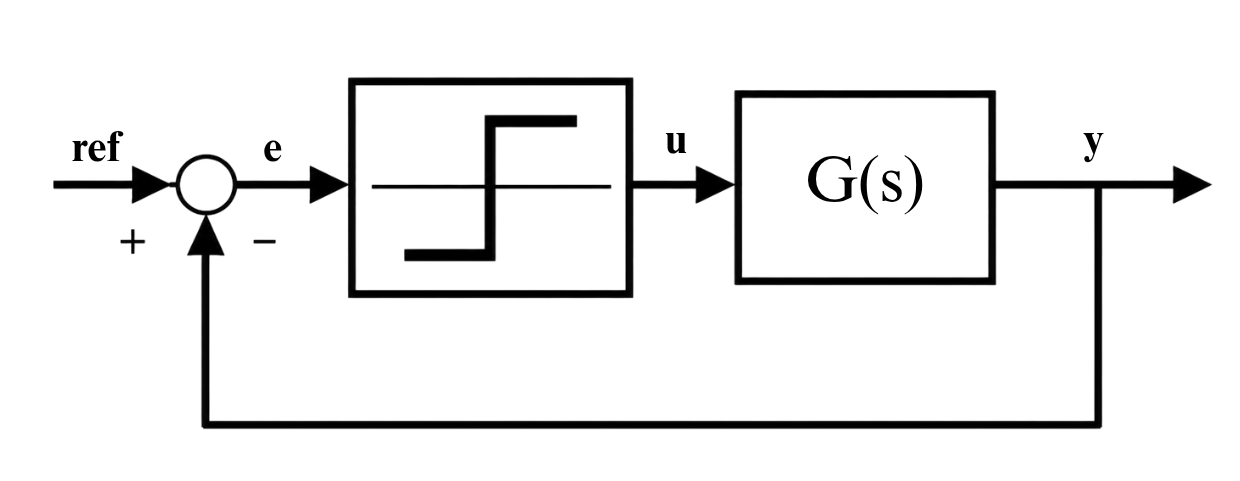
\includegraphics[width=9cm]{figuras/fundamentação-teorica/block-diagram-relay.png}
				}{
					\Fonte{O autor}
				}	
			\end{figure}

			\begin{figure}[htb]
				\centering
				\Caption{\label{fig:sinal-saida-rele} Resposta desejada com o uso do Relé}
				\UFCfig{}{
					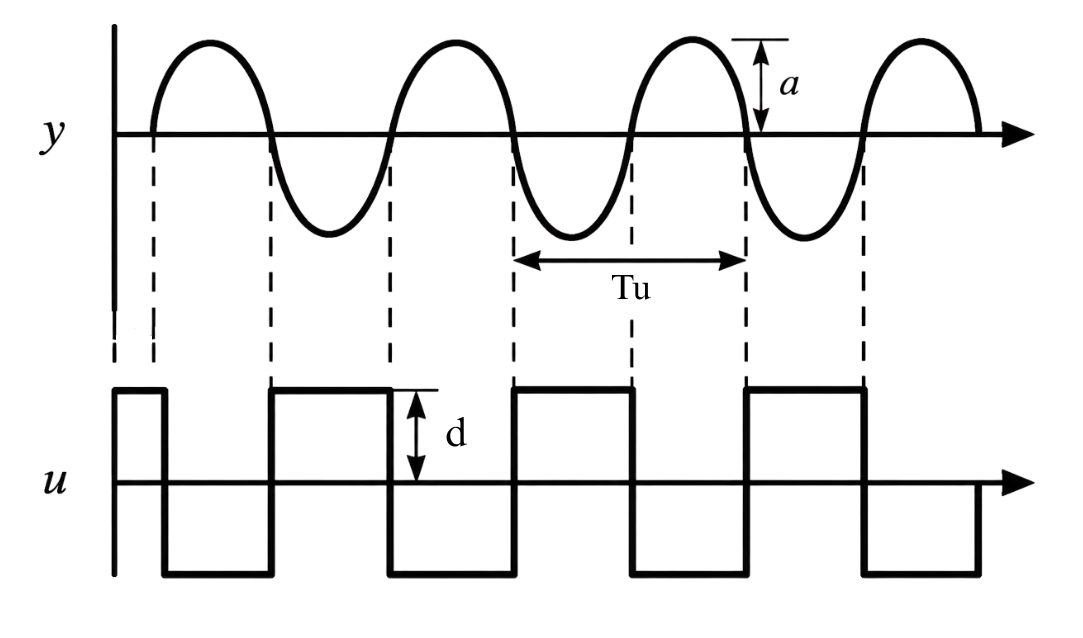
\includegraphics[width=9cm]{figuras/fundamentação-teorica/output-relay.png}
				}{
					\Fonte{O autor}
				}	
			\end{figure}

			Tradicionalmente, o segundo método de \gls{ZN} propõe a adição de um bloco Controlador Proporcional no diagrama da Figura \ref{fig:sistema-malha-fechada-controlador} para que com o aumento do ganho $K_p$ o sistema apresente oscilações até o momento em que atinja o limiar de estabilidade, ou seja, fique completamente oscilatório e nesse momento o valor do ganho atinge seu valor que é dito \textit{crítico} (ou último), $K_u$. São medidos, também, o período da oscilação, $T_u$, e a frequência de oscilação $\omega_u$. 
			
			De posse dessas medidas tal método propõe a utilização da Tabela \ref{tab:zn2-parametros} para a determinação dos valores de $K_p$, $T_i$ e $T_d$. Todavia, em diversos processos, a aplicação direta do método descrito anteriormente não é viável, uma vez que as condições operacionais não permitem o aumento progressivo do ganho até que se atinja o \textit{ganho crítico}.

			\begin{table}[!htbp]	
				\centering
				\Caption{\label{tab:zn2-parametros} Sintonia de controladores \gls{PID} pelo segundo método de \gls{ZN}}
				\UFCtab{}{
					\begin{tabular}{cccc}
						\toprule
						Tipo de controlador & \( K_p \) & \( T_i \) & \( T_d \) \\
						\midrule
						P    & \( 0,5 K_{u} \) & \( \infty \) & \( 0 \) \\
						PI   & \( 0,45 K_{u} \) & \( \frac{1}{1,2} T_{u} \) & \( 0 \) \\
						PID  & \( 0,6 K_{u} \) & \( 0,5 T_{u} \) & \( 0,125 T_{u} \) \\
						\bottomrule
					\end{tabular}
				}{
					\Fonte{\citeonline{ogata-2010}}
				}
			\end{table}

			% Todavia, em diversos processos não é possível a aplicação direta do método acima descrito haja vista que as condições operacionais não permitirão ao aumento progressivo do ganho até se alcançar o \textit{ganho crítico}. Dessa forma, {\AA}str{\"o}m e H{\"a}gglund propõem a utilização de um relé para se alcançar tais parâmetros. E, assim, quando este é introduzido, o sistema passa automaticamente a oscilar com período $T_u$ e freqûencia $\omega_u$ as quais possuem a seguinte relação: 
			
			% \citeonline{astrom-1995} observaram que com a introdução de um relé de amplitude $d$, na malha de controle, o sistema produz uma saída oscilatória de amplitude $a$ (Figura \ref{fig:sinal-saida-rele}), automaticamente, com período $T_u$ e frequência $\omega_u$, os quais estão relacionados conforme a equação \ref{eq:relacao-periodo-frequencia}. O valor do \textit{ganho crítico}, por sua vez, está relacionado com a amplitude do relé e com a amplitude do sinal de saída, conforme a equação \ref{eq:ganho-critico-rele}. 
			
			\citeonline{astrom-1995} observaram que a introdução de um relé de amplitude $d$ na malha de controle faz com que o sistema produza automaticamente uma saída oscilatória com amplitude $a$ (Figura \ref{fig:sinal-saida-rele}). Essas oscilações ocorrem com período $T_u$ e frequência $\omega_u$, relacionadas pela Equação \ref{eq:relacao-periodo-frequencia}. Além disso, o valor do \textit{ganho crítico} está diretamente relacionado à amplitude do Relé e à amplitude do sinal de saída, conforme expresso na Equação \ref{eq:ganho-critico-rele}.


			\begin{equation}
				\label{eq:relacao-periodo-frequencia}
				\omega_u = \frac{2 \pi}{T_u}
			\end{equation}

			\begin{equation}
				\label{eq:ganho-critico-rele}
				K_u = \frac{4 d}{\pi a}
			\end{equation}

			% Assim, considerando a curva de Nyquist pode-se entender o Relé como sendo o elemento que desloca um ponto na curva característica do processo para uma posição desejada. É possível, ainda, considerar uma histerese $\epsilon$ para que o ponto na curva seja deslocado no plano complexo.

			Considerando o diagrama de \textit{Nyquist}, o Relé pode ser interpretado como um elemento que desloca o ponto de operação associado à oscilação para uma posição específica na curva característica do processo. Além disso, é possível introduzir uma histerese $\varepsilon$, modificando sua característica de chaveamento. A presença dessa histerese permite deslocar o ponto correspondente na curva de \textit{Nyquist} para uma nova posição no plano complexo, ampliando a flexibilidade do método na obtenção das informações dinâmicas do processo. Dessa forma, é possível explorar diferentes regiões da curva característica, possibilitando uma manipulação mais abrangente do comportamento do sistema. 
			
			A Equação característica do \textit{Relé com Histerese}, \ref{eq:equacao-rele-histerese}, a seguir, mostra que o sem a histerese ($\varepsilon = 0$) o ponto da curva de \textit{Nyquist} se encontrava em cima do eixo real, em seu lado negativo. Com ela o ponto passa a ser deslocado agora para o $3^\circ$ quadrante do plano complexo.

			\begin{equation}
				\label{eq:equacao-rele-histerese}
				G(j \omega) = -\frac{1}{N(a)} = -\frac{\pi}{4d} \sqrt{a^2 - \varepsilon^2} - j \frac{\pi \varepsilon}{4d}
			\end{equation}

			\noindent
			onde, 

			\begin{equation*}
				\begin{cases}
					\operatorname{Re}\{G(j \omega)\} = -\dfrac{\pi}{4d} \sqrt{a^2 - \varepsilon^2} \\[10pt]
					\operatorname{Im}\{G(j \omega)\} = -\dfrac{\pi \varepsilon}{4d}
				\end{cases}
			\end{equation*}

			O ponto encontrado pode ser então descrito pelo seu módulo $R_a$ e sua fase $\phi_a$ dados pelas Equações \ref{eq:modulo-rele} e \ref{eq:fase-rele}, respectivamente.

			\begin{equation}
				\label{eq:modulo-rele}
				R_a = \sqrt{(\operatorname{Re}\{G(j \omega)\})^2 - (\operatorname{Im}\{G(j \omega)\})^2}
			\end{equation}

			\begin{equation}
				\label{eq:fase-rele}
				\phi_a = \arctan \left( \frac{\operatorname{Im}\{G(j \omega)\}}{\operatorname{Re}\{G(j \omega)\}} \right)
			\end{equation}

			O controlador \gls{PID}, descrito pela Equação \ref{eq:definicao-pid-laplace} provoca um novo deslocamento em fase e módulo do ponto na curva de \textit{Nyquist}, encontrando um novo ponto agora com módulo $R_b$ e fase $\phi_b$. À variação sofrida dá-se o nome, respectivamente, de margem de fase $\phi_m$ e margem de ganho $A_m$ os quais podem ser descritos pelas Equações \ref{eq:margem-fase} e \ref{eq:margem-ganho}.

			\begin{equation}
				\label{eq:margem-fase}
				\phi_m = \phi_b - \phi_a
			\end{equation}

			\begin{equation}
				\label{eq:margem-ganho}
				A_m = \frac{R_b}{R_a}
			\end{equation}

			E assim, os parâmetros de controle $K_p$, $T_i$ e $T_d$ podem ser definidos conforme \citeonline{astrom-1984} em função dos elementos já apresentados e de um novo valor $\alpha$.

			\begin{equation}
				\label{eq:parametro-kp}
				K_p = \frac{K_u}{A_m} \cos \phi_m
			\end{equation}

			\begin{equation}
				\label{eq:parametro-td}
					T_d = \frac{\tan \phi_m + \sqrt{\frac{4}{\alpha} + \tan^2 \phi_m}}{2 \omega_u}
			\end{equation}

			\begin{equation}
				\label{eq:parametro-ti}
				T_i = \alpha T_d
			\end{equation}

			Dessa forma, serão projetados controladores do tipo \gls{PID} para o robô \textit{micromouse}, considerando os processos anteriormente descritos. A partir dos parâmetros obtidos pelos métodos de sintonia apresentados, busca-se determinar ajustes adequados para cada malha de controle, de modo a atender aos requisitos de desempenho necessários para o sistema.

%%%%%%%%%%%%%%%%%%%%%%%%%%%%%%%%%%%%%%%%%%%%%%%%%%%%%%%%%%%%%%%%%%%%%%%%%%%%%%%%%%%%%%%%%%%%%%%%%%%%%%%%%%%%%%%%%%%%%%%%%%%%%%%%%%%%%%

\chapter{O Micromouse}
\label{cap:micromouse}

Os robôs móveis têm obtido mais relevância nas últimas décadas com o aprimoramento da microeletrônica e da programação. Estes robôs consistem em sistemas embarcados com microcontroladores e diversos tipos de sensores para se obter as mais variadas informações, sendo os mais comuns os que trabalham com distância, velocidade e angulação. Os sensores podem, ainda, ser classificados em dois grupos: os sensores internos, os quais ficam na própria planta, e os sensores externos, colocados no ambiente de atuação do robô \cite{dissetacao-pereira-2000}.


    \section{Características Construtivas} \label{sec:caracteristicas-construtivas}
		Conforme apresentado em \citeonline{manual-microumouse-2015} o robô \textit{$\mu$MaRT Lite Plus} faz parte de um kit de aprendizado de robótica, dispondo do microcontrolador STM32F405RGT6. O robô, que daqui para frente será chamado apenas de \textit{micromouse}, dispõe ainda de 3 botões, sendo um botão de \textit{boot}, um de \textit{reset} e um botão configurável, além de sensores de linha (oito ao total), sensores de parede (quatro ao total), um conector \gls{USB}, um conector \gls{UART}, dois motores com um \textit{encoder} cada, \textit{buzzer} para sinalização sonora, medição de tensão de bateria, um giroscópio para medir a orientação do robô e duas chaves Liga/Desliga sendo uma geral e uma para os motores. A Figura \ref{fig:micromouse-composicao} apresenta uma vista superior do micromouse e da sua composição.
        
		\begin{figure}[htbp]
                \centering
                \Caption{\label{fig:micromouse-composicao} Estrutura e composição do \textit{micromouse}}	
                \UFCfig{}{
                    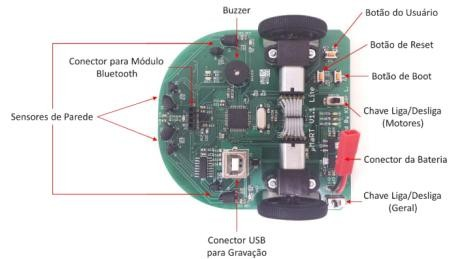
\includegraphics[width=14cm]{figuras/fundamentação-teorica/composicao_micromouse.jpg}
                }{
                    \Fonte{\citeonline{manual-microumouse-2015}}
                }	
        \end{figure}

		\subsection{Programação e Bootloader} \label{ssec:programacao-e-bootloader}
			A programação e gravação dos códigos embarcados (\textit{bootloader}) no robô \textit{micromouse} seguem conforme instruções do desenvolvedor em \citeonline{manual-config-bootloader}, \citeonline{manual-criacao-arm-project}, \citeonline{manual-config-eclipse}  e \citeonline{manual-microumouse-2015}.

	\section{Cinemática} \label{sec:cinematica-micromouse}
		Uma característica fundamental para entender o comportamento do \textit{micromouse} é a sua tração diferencial, isto é, devido ao movimento independente dos seus motores, a sua posição e velocidade global será definida pela diferença de velocidade entre as rodas esquerda e direita. A Figura \ref{fig:movimento-diferencial-micromouse} a seguir ilustra o comportamento descrito anteriormente.

		\begin{figure}[htbp]
                \centering
                \Caption{\label{fig:movimento-diferencial-micromouse} Comportamento diferencial do \textit{micromouse}}	
                \UFCfig{}{
                    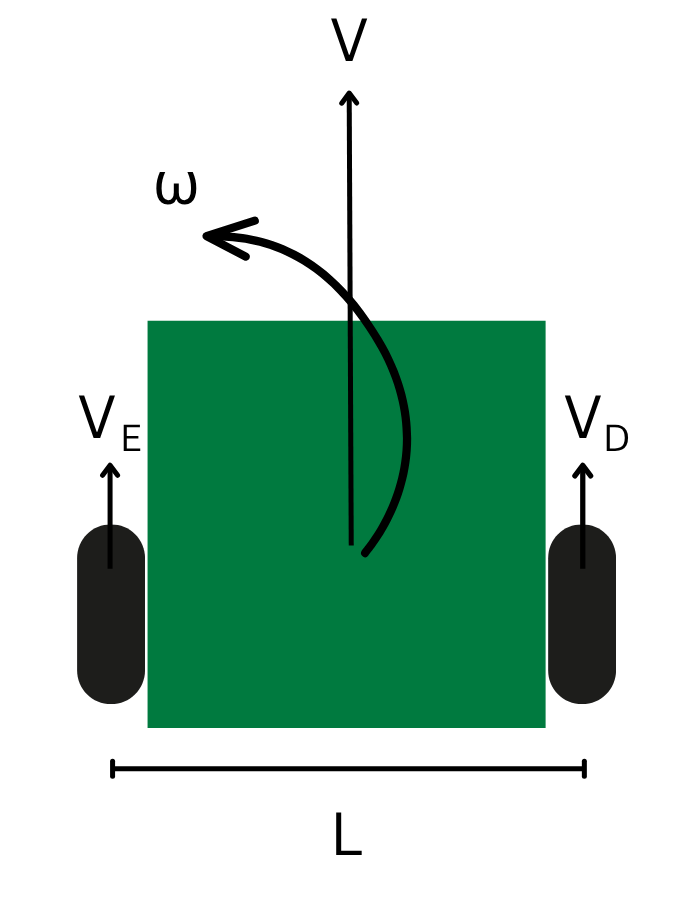
\includegraphics[width=5cm]{figuras/fundamentação-teorica/mov-diferencial-micromouse-puro.png}
                }{
                    \Fonte{O autor}
                }	
        \end{figure}

		Dessa forma a velocidade linear global (\textit{V}) e a velocidade angular global ($\omega$) podem ser calculadas a partir das Equações \ref{eq:vel-linear-global} e \ref{eq:vel-angular-global} e estão apresentadas no formato das Equações \ref{eq:vel-linear-direita} e \ref{eq:vel-linear-esquerda}.

		\begin{equation}
			\label{eq:vel-linear-global}
			V = \frac{V_D + V_E}{2}
		\end{equation}

		\begin{equation}
			\label{eq:vel-angular-global}
			\omega = \frac{V_D - V_E}{L}
		\end{equation}

		\begin{equation}
			\label{eq:vel-linear-direita}
			V_D = \frac{2V + L\omega}{2}
		\end{equation}

		\begin{equation}
			\label{eq:vel-linear-esquerda}
			V_E = \frac{2V - L\omega}{2}
		\end{equation}

		Assim, pode-se notar que as velocidades dependem diretamente da geometria do robô de forma que algumas considerações devem ser feitas:

		\begin{alineas}
			\item Os modelos apresentados nas Equações \ref{eq:vel-linear-global}, \ref{eq:vel-angular-global} não são a única forma de modelar a cinemática do robô. \citeonline{deshmukh-hasamnis-2023}, por exemplo, utilizam um modelo ligeiramente diferente considerando uma nova variável \textbf{R} (raio do centro instatâneo da curva) no denominador das equações citadas;
			
			\item O modelo apresentado em \ref{eq:vel-angular-global} considera o sentido \textbf{positivo} de giro sendo o sentido \textbf{anti-horário};
		\end{alineas}

		Assim, o comportamento cinemático do micromouse, pode ser representado em um diagrama de blocos, ilustrado a seguir na Figura \ref{fig:diagrama-blocos-micromouse}.

		\begin{figure}[htbp]
                \centering
                \Caption{\label{fig:diagrama-blocos-micromouse} Diagrama de blocos da cinemática do \textit{micromouse}}	
                \UFCfig{}{
                    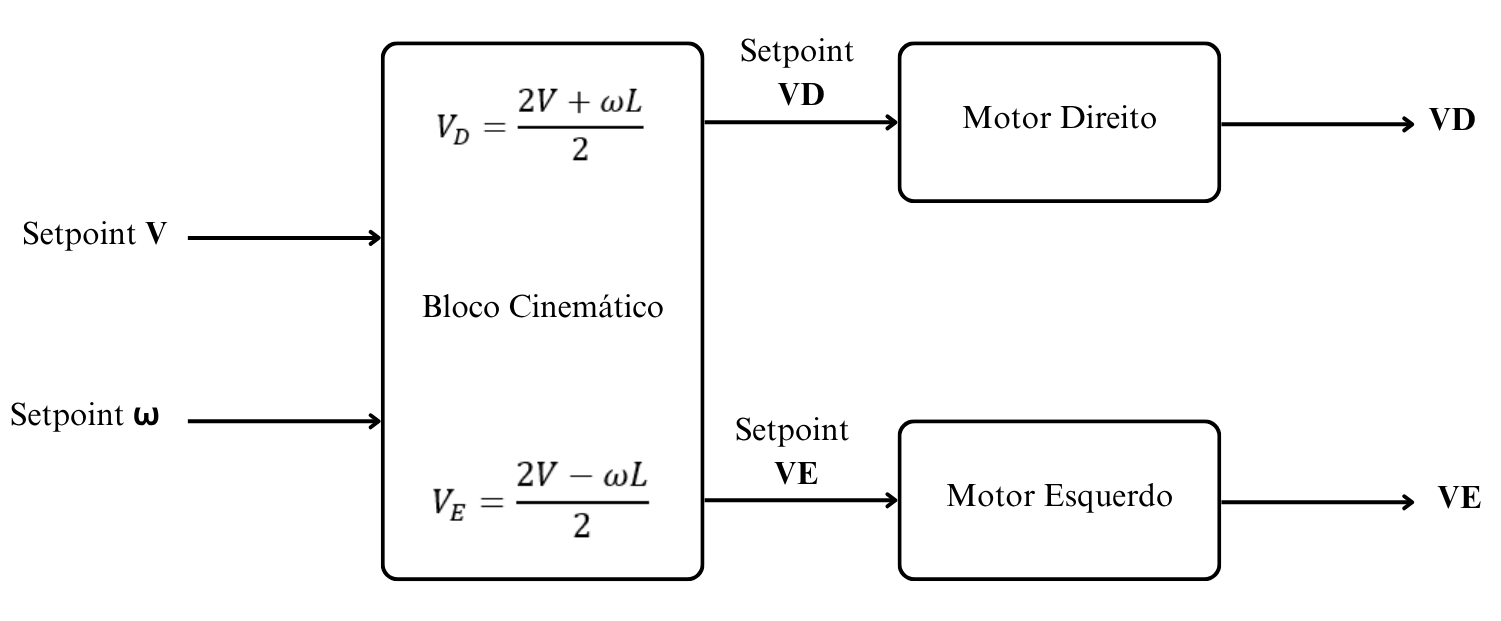
\includegraphics[width=12cm]{figuras/fundamentação-teorica/diagrama-bloco-micromouse.png}
                }{
                    \Fonte{O autor}
                }	
        \end{figure}

	\section{Posicionamento e Orientação} \label{sec:posicionamento-e-orientacao}
		
		Um aspecto imprescindível para a realização do rastreio de trajetórias é o conhecimento sobre a posição atual do robô \textit{micromouse} em cada instante de amostragem de forma a fornecer informações para correções da movimentação. Como no presente trabalho não se dispõe de mecanismos de supervisão externa para acompanhamento, como ocorre em \citeonline{dissetacao-pereira-2000}, tais informações devem ser obtidas com os dados fornecidos pelos sensores do robô e as equações pertinentes de posicionamento devem ser desenvolvidas a partir das equações cinemáticas anteirores.

		De posse das Equações \ref{eq:vel-linear-global} a \ref{eq:vel-linear-esquerda} pode-se obter a representação matricial da cinemática do robô, dada pela Equação \ref{eq:matriz-cinematica-micromouse} onde $\dot{x}_c$, $\dot{y}_c$ e $\dot{\theta}$ representam as variações de posição na direção $x$, $y$ e a variação de orientação $\theta$ respectivamente, como indicado em \ref{fig:micromouse-plano-cartesiano}.

		\begin{equation}
			\label{eq:matriz-cinematica-micromouse}
			\begin{bmatrix}
			\dot{x}_c \\
			\dot{y}_c \\
			\dot{\theta}
			\end{bmatrix}
			=
			\begin{bmatrix}
			\cos\theta & 0 \\
			\sin\theta & 0 \\
			0 & 1
			\end{bmatrix}
			\begin{bmatrix}
			v \\
			\omega
			\end{bmatrix}
		\end{equation}

		\begin{figure}[htbp]
			\centering
			\Caption{\label{fig:micromouse-plano-cartesiano} Deslocamento no plano cartesiano do \textit{micromouse}}	
			\UFCfig{}{
				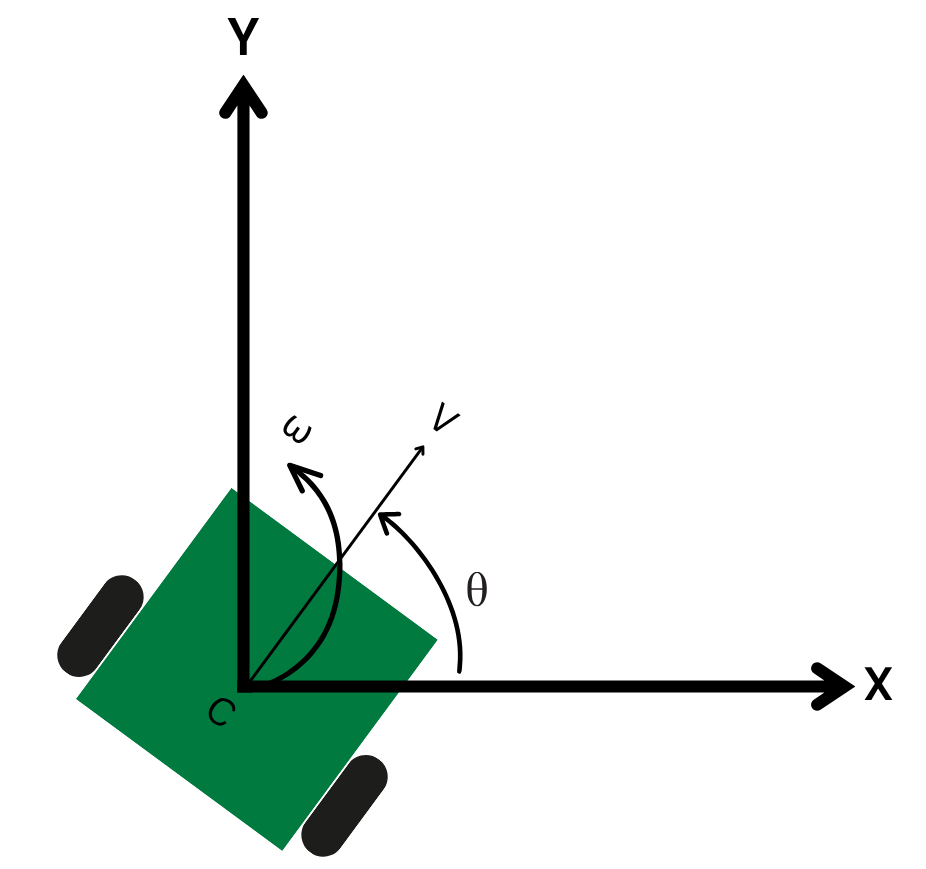
\includegraphics[width=4cm]{figuras/fundamentação-teorica/micromouse-no-plano.png}
			}{
				\Fonte{O autor}
			}	
		\end{figure}

		% Assim, estabelece-se a restrição de movimento do robô \textit{micromouse}, a chamada restrição \textbf{não-holonômica}, a qual implica que o robô não pode se mover em qualquer direção, ou seja, mecanicamente implica queele não pode se descolcar com velocidade perpendicular à posição das suas rodas. A restrição não-holonômica é definida pela equação \ref{eq:restricao-nao-holonomica}.

		Assim é estabelecida a restrição de movimento característica do robô \textit{micromouse}, denominada restrição \textbf{não holonômica}. Essa restrição decorre da configuração do robô diferencial e implica que seu movimento não pode ser realizado de forma arbitrária em todas as direções do plano. 
		
		Em termos físicos, isso significa que o robô não é capaz de desenvolver velocidade lateral instantânea, ou seja, não pode se deslocar perpendicularmente ao plano de rotação de suas rodas sem que haja previamente uma mudança em sua orientação. Dessa forma, seus movimentos ficam limitados às direções compatíveis com sua estrutura mecânica e com as condições de rolamento impostas pelas rodas \cite{vieira-2005}. 
		
		Matematicamente, essa restrição é descrita pela equação \ref{eq:restricao-nao-holonomica}.
		
		\begin{equation}
			\label{eq:restricao-nao-holonomica}
			\dot{x}\,\sin(\theta) - \dot{y}\,\cos(\theta) = 0
		\end{equation}
